%!TEX TS-program = xelatex
%
% Created by Chris on 2020-07-30.
% Copyright (c) Chris von Csefalvay, 2020.
\documentclass{article}
\usepackage{amsmath}
\usepackage{amsfonts}


% Bibliography styling
\usepackage[super,square,sort&compress,numbers]{natbib}
\bibliographystyle{unsrtnat}

% Define eqdef operator
\newcommand{\eqdef}{\overset{\mathrm{def}}{=\joinrel=}}

% Graphics
\usepackage{graphicx}

\title{Time series classification of COVID-19 dynamics in the United States}
\author{Chris von Csefalvay\thanks{Starschema Inc., Arlington, VA. Correspondence: \texttt{csefalvayk@starschema.net}.}}

\begin{document}

\maketitle

\begin{abstract}
    The statistical dynamics of a pathogen within a population depend on a range of factors: population density, the effectiveness and investment into social distancing, public policy measures and non-pharmaceutical interventions (NPIs) are only some examples of factors that influence the number of cases over time. This paper outlines a time series cluster analysis of confirmed COVID-19 cases in the United States, using a soft-DTW (Dynamic Time Warping) k-means clustering and a k-shape based clustering algorithm to identify internally consistent clusters of case counts over time. The identification of disjoint time series clusters can use past patterns to discern the future of infectious dynamics in an area, and through identifying the most likely cluster-wise trajectory, inform public health decision-making.
\end{abstract}


\section{Introduction} % (fold)
\label{sec:introduction}

The emergence of SARS-CoV-2, and its associated viral syndrome COVID-19, has raised important questions about the ways we analyse and identify dynamic temporal processes. In particular, by identifying similarities in principal time-dependent indicators of epidemic dynamics, such as prevalence (the number of confirmed cases over time), we can gain insight into similarities that are likely to emerge across various regions. Through this, time series clustering has the potential to play a significant role in understanding the dynamic processes that drive an outbreak.

Clustering is the wider set of algorithms within unsupervised learning that identify similar patterns among data in arbitrarily high-dimensional spaces, effectively taking a set $\mathcal{P}$ of $N$ vectors in an $n$-dimensional space, and assigning to each of these a label from the set $\mathcal{L}$, so that the assignment of each element of $\mathcal{P}$ to the groups defined by the labels comprising $\mathcal{L}$ minimise some objective function (typically referred to as the distance metric of the clustering). Cluster algorithms are widely used today and their practical applications are ubiquitous, ranging from identifying clinical phenotypes in clinical medicine\cite{ahmad2014clinical,haldar2008cluster,lochner2005cluster,weatherall2009distinct,ye2014different} through fraud detection\cite{behera2015credit,liu2013healthcare,peng2006application,sabau2012survey,subudhi2017use} to image segmentation.\cite{chuang2006fuzzy,coleman1979image,jin2018accelerating,lafata2018data,pappas1989adaptive,wu1993optimal}

Time series clustering presents a particular complication of this problem insofar as the subject of clustering is not a vector representing a single value, but rather a time series. These time series are typically not in synchrony, but rather exhibit a range of delays, lags and leads, and may depend on extrinsic hidden variables. We may formulate the essential task of time series clustering as follows. Let $X$ comprise $n$ time series $x_{1 \ldots n}$, and let $k$ denote the cardinality of the set $\mathcal{L}$ -- in other words, the number of partitions we wish to split the data into, with $k \leq n$. Then, the mapping $f: X \rightarrow l \ | \ l \in \mathcal{L}$ is a clustering if it assigns to any element $x_i \in X \ | \ i \leq n$ one (and only one) cluster $l_i \in \mathcal{L}$, so as to minimise an objective function (typically referred to in this context as a distance metric) $J$ within the cluster.

This paper examines the use of two time series clustering algorithms -- soft-DTW k-means clustering and k-shape clustering -- to identify different patterns in COVID-19 prevalence in the continental United States, and comparing the results of the classifiers for inter-classifier consistency. By isolating the barycenters of the time-shifted clusters, we can identify consistent patterns in prevalence dynamics across multiple states, quantifying the overall effect of pre-existing characteristics, population dynamics and non-pharmaceutical interventions (NPIs) between states.

% section introduction (end)

\section{Methods} % (fold)
\label{sec:methods}

\subsection{Source data} % (fold)
\label{sub:source_data}

Source data for the 48 states of the continental United States was obtained from the Starschema COVID-19 Data Set,\cite{foldi_tamas_2020_3969287} and filtered only for confirmed case counts. Data was loaded into Python 3.7 using \texttt{pandas},\cite{mckinney2011pandas} and values were scaled using \texttt{tslearn.preprocessing}'s \texttt{TimeSeriesScalerMeanVariance} to $\mu = 0$ and $\sigma = 1$. The results of this transformed raw data set are laid out, by state, in Figure~\ref{fig:scaled_by_state}. 

\begin{figure}
	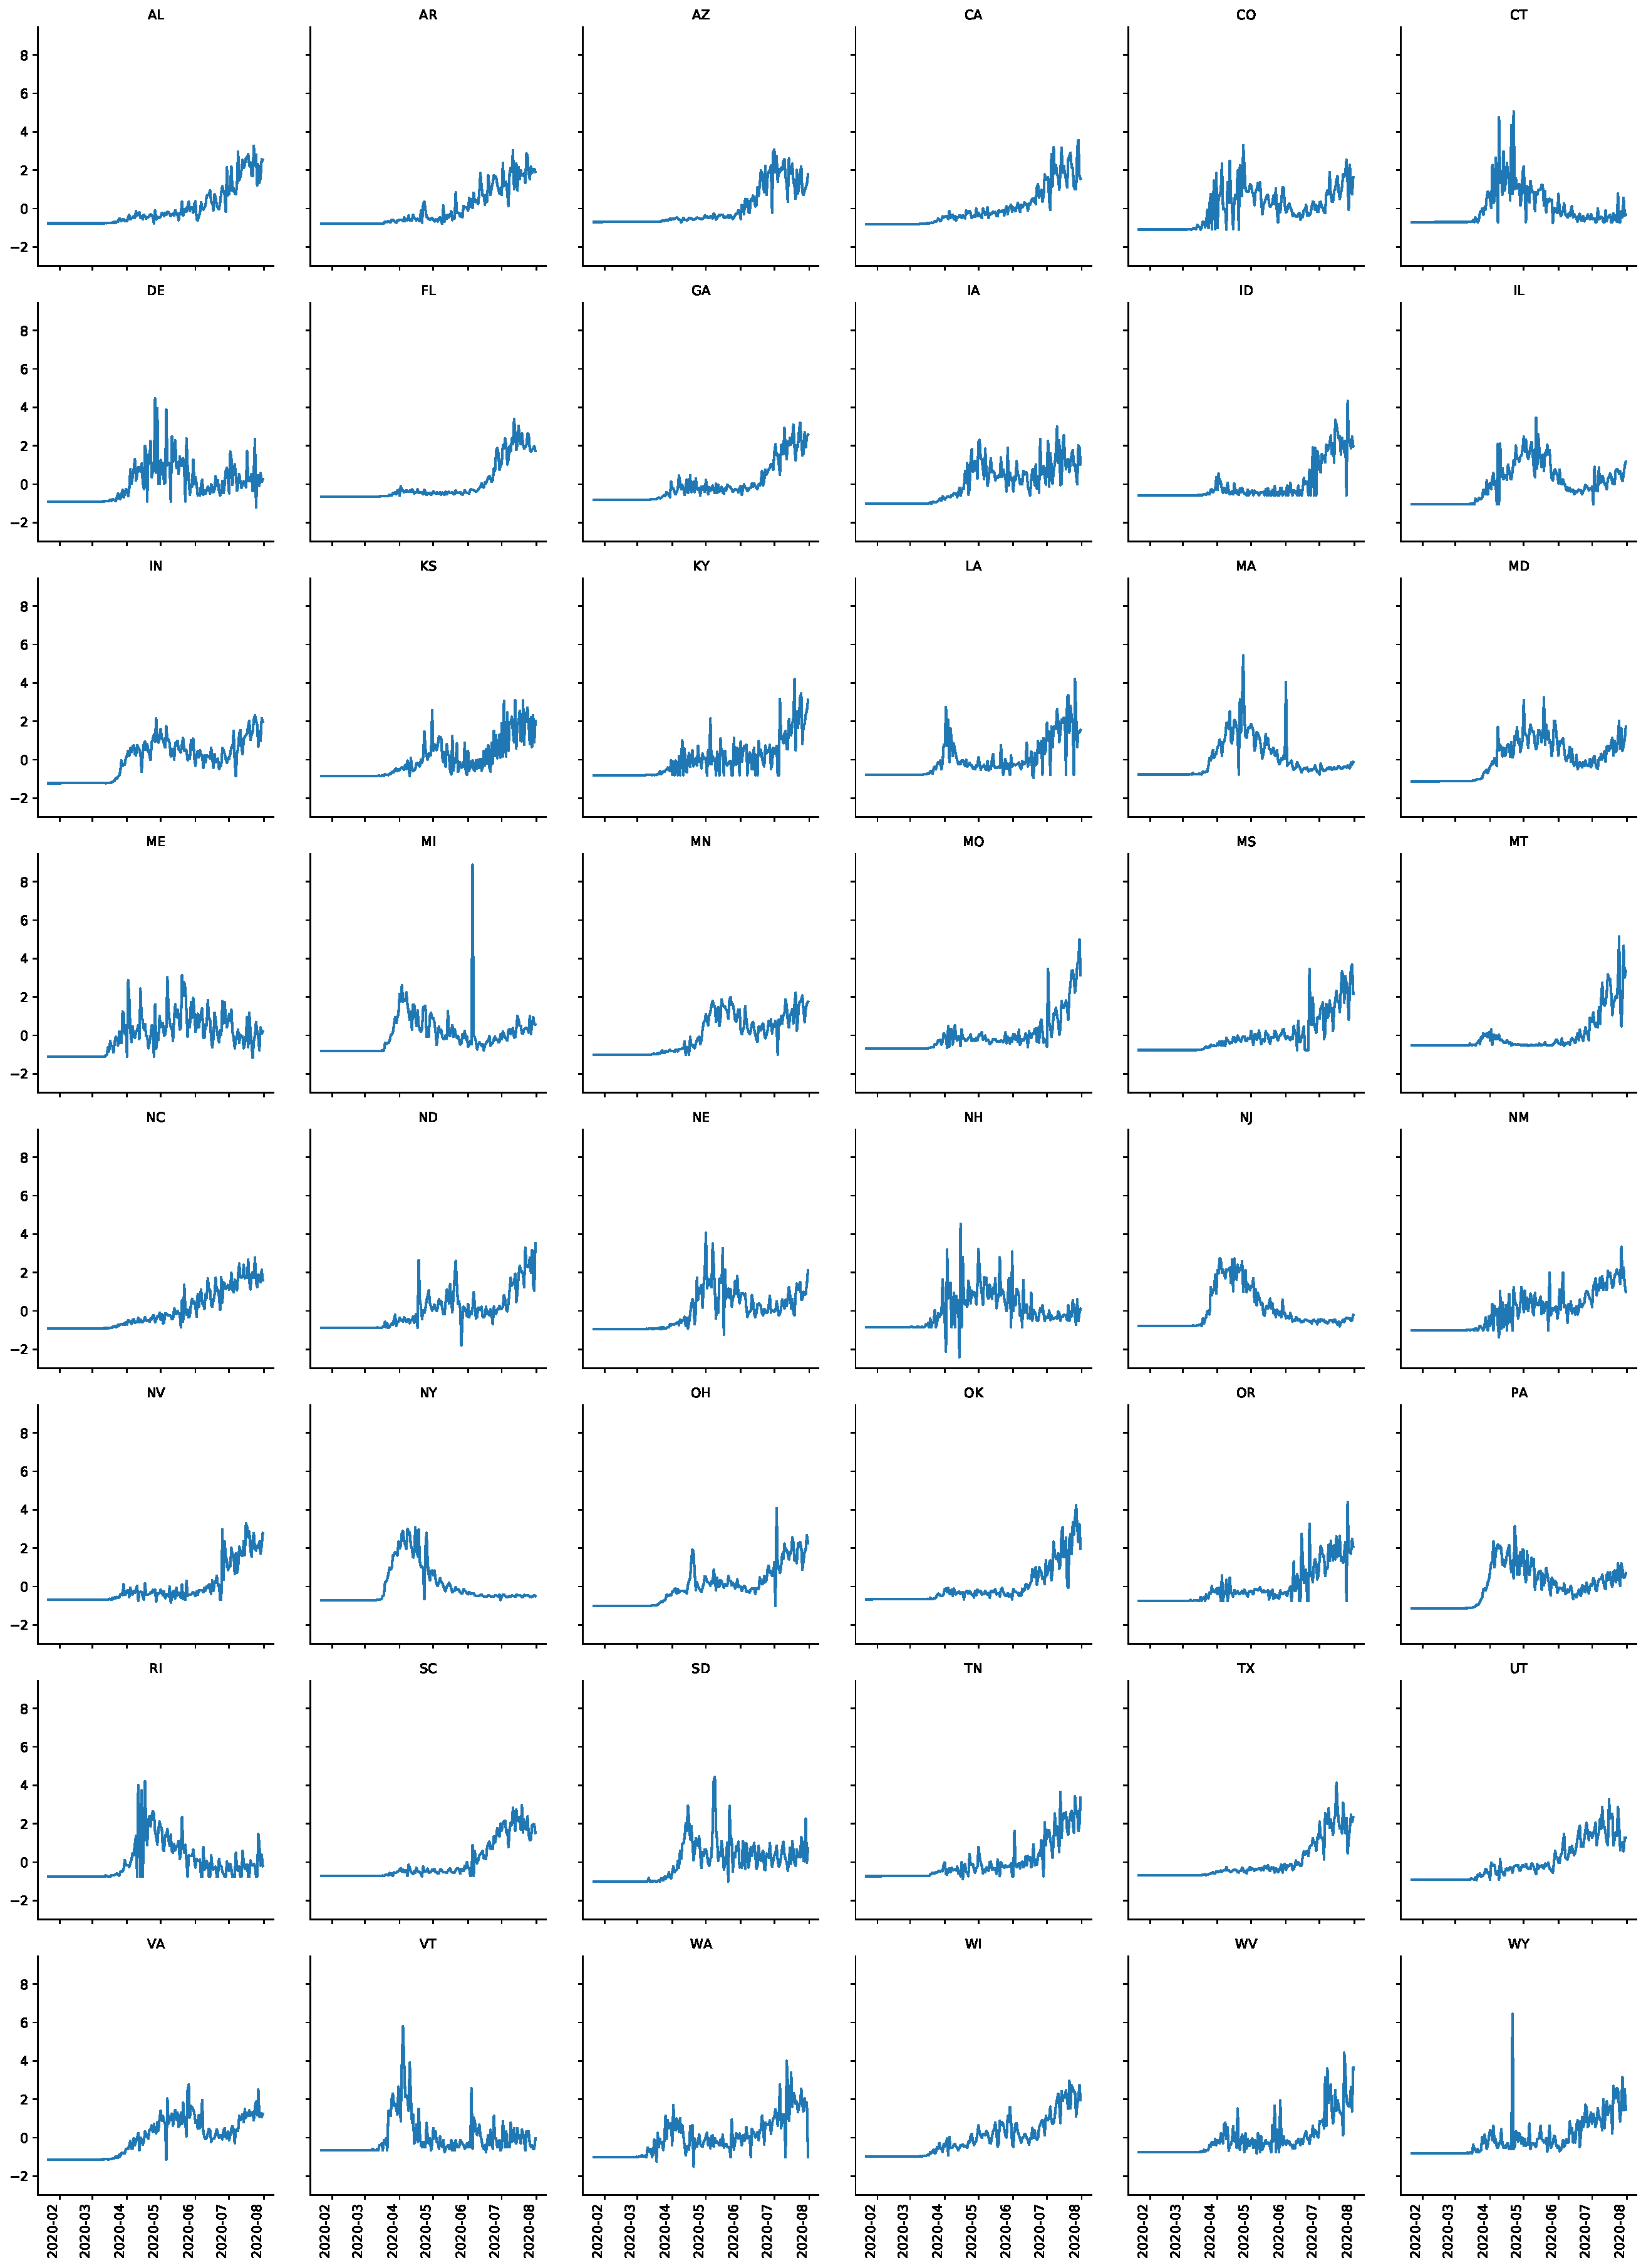
\includegraphics[width=\linewidth]{figures/scaled-by-state}
	\centering
	\caption{Scaled raw data of prevalence by state.}
	\label{fig:scaled_by_state}
\end{figure}

% subsection source_data (end)

\subsection{Soft-DTW k-means clustering} % (fold)
\label{sub:soft_dtw_k_means_clustering}

Since first described by Sakoe and Chiba (1978),\cite{sakoe1978dynamic} the dynamic time warping algorithm has been expressed in multiple formulations. The presentation below is based on Cuturi and Blondel's 2017 paper introducing Soft-DTW, with the marginal difference of using $J(\cdot, \cdot)$ instead of $\delta$ to represent the distance function.\cite{cuturi2017soft} 

Given two time series $x_t: t_x \in \mathbb{Z}$ and $y_t: t_y \in \mathbb{Z}$, there exists a cost matrix $\Delta(\mathbf{x}, \mathbf{y})$ for the distance function $J$, from which we can derive the cost matrix 

\begin{equation}
	\Delta(\mathbf{x}, \mathbf{y}) = [J(x_i, y_j)]_{ij} \in \mathbb{R}^{t_x \times t_y} 
\end{equation}

For the two above-mentioned series, we describe the set of matrices of all possible alignments as $\mathcal{A}_{t_x, t_y}$, which is a strict subset of $\{0, 1\}^{t_x \times t_y}$. Then, DTW can be defined as the function that for any pair $(\mathbf{x}, \mathbf{y})$ identifies $A \in \mathcal{A}_{t_x, t_y}$ so as to minimise the inner product of A with the cost matrix $\Delta(\mathbf{x}, \mathbf{y})$.

\begin{equation}
	DTW(\mathbf{x}, \mathbf{y}) \eqdef \min_{A \in \mathcal{A}_{t_x, t_y}} \langle A_{t_x, t_y}, \Delta(\mathbf{x}, \mathbf{y})
\end{equation}

Thus, DTW can be conceived of as a search task, in which $\mathcal{A}_{t_x, t_y}$ is the search space within which we search for $A$ so as to minimise $\langle A, \Delta(\mathbf{x}, \mathbf{y}) \rangle$. 

Soft-DTW universalises the notion underlying the DTW cost metric and the global alignment kernel metric

\begin{equation}
	GAK_{\gamma}(\mathbf{x}, \mathbf{y}) \eqdef \sum_{A \in \mathcal{A}_{t_x, t_y}} e^{- \frac{\langle A, \Delta(\mathbf{x}, \mathbf{y} \rangle)}{\gamma}}
	\label{eq:gak}
\end{equation}

\noindent into a single metric.\cite{janati2020spatio} Given the generalisation of the minimum metric with a smoothing factor $\gamma \geq 0$,

\begin{equation}
	\min^{\gamma} \{a_{1 \ldots n}\} \eqdef 
	\begin{cases}
		\displaystyle \min_{i \leq n} a_i, 								& \gamma = 0 \\
		- \gamma \log \displaystyle \sum_{i=1}^n e^{-\frac{a_i}{\gamma}},	& \gamma > 0
	\end{cases}
\end{equation}

\noindent we may now define Soft-DTW as

\begin{equation}
	sDTW_{\gamma}(\mathbf{x}, \mathbf{y}) \eqdef \min_{A \in \mathcal{A}_{t_x, t_y}} ^{\gamma} \{ \langle A, \Delta(\mathbf{x}, \mathbf{y}) \rangle \}
\end{equation}

Importantly, Soft-DTW -- unlike the original DTW approach by Sakoe and Chiba\cite{sakoe1978dynamic} -- is explicitly differentiable. In particular, as Saigo (2006) noted,\cite{saigo2006optimizing} the gradient of 
 Equation~\eqref{eq:gak} can be calculated quite conveniently. Let $\hat{A}$ be the average alignment matrix following the Boltzmann distribution $p_{\gamma} \sim e^{- \langle A_i, \frac{\Delta(\mathbf{x}, \mathbf{y}) \rangle}{\gamma}}$ for all $A_i \in \mathcal{A}_{t_x, t_y}$. Then, 
 
\begin{equation}
 	\hat{A} = \frac{\displaystyle \sum_{A_i \in \mathcal{A}_{t_x, t_y}} A_i e^{- \langle A, \frac{\Delta(\mathbf{x}, \mathbf{y})}{\gamma}\rangle}}{GAK_{\gamma}(\mathbf{x}, \mathbf{y})}
 \end{equation}

\noindent and consequently

\begin{equation}
	\nabla_{\mathbf{x}} DTW_{\gamma} (\mathbf{x}, \mathbf{y}) = \Bigg( \frac{\partial \Delta(\mathbf{x}, \mathbf{y})}{\partial \mathbf{x}} \Bigg)^T \hat{A}
\end{equation}

This can be easily calculated using backward recursion, as described in Algorithm 2 of Cuturi and Blondel (2017).\cite{cuturi2017soft} In addition, the notion of a clustering centroid can be generalised to the metric space comprising the time series to yield Fr\^{e}chet means, also referred to in this context as barycenters. For a metric space $(M, \tau)$, $p \in M$ is a Fr\^{e}chet mean of order $q \geq 1$ of the time series $x_{1 \ldots n} \in M$ if it minimises the Fr\^{e}chet variance, i.e.

\begin{equation}
	p = \mathop{arg min}_{r \in M} \sum_{j = 1}^n \tau(x_j, r)^q
\end{equation}

Based on dynamic time warping distances between temporal signals, we can construct a clustering that divides the COVID-19 prevalence time series for the 48 states of the contiguous United States into a number of clusters so as to minimise distances using k-nearest neighbour clustering. Soft-DTW clustering was performed using \texttt{tslearn} 0.4.1\cite{JMLR:v21:20-091} using Python 3.7, with a $\gamma$ parameter of $0.1$.

% subsection soft_dtw_k_means_clustering (end)

\subsection{k-shape clustering} % (fold)
\label{sub:k_shape_clustering}

k-shape clustering is a novel, robust clustering algorithm for time series that relies on iteratively refining clusters, with cross-correlation as the underlying distance metric.\cite{paparrizos2015k} Specifically, k-shape relies on a normalised version of cross-correlation, referred to in this context as Shape Base Distance (SBD): time series are Z-normalised (i.e. $\mu = 0$ and $\sigma = 1$), and the resulting cross-correlation sequence is divided by the geometric mean of the individual time series' autocorrelations. In this sense, k-shape can be understood as a k-means clustering that uses a cross-correlation based metric $SBD(\mathbf{x}, \mathbf{y})$. Let $mathbf{x}_s$ be the series $\mathbf{x}$ shifted, with zero-padding, by s, and the same be true for $mathbf{y}_s$ respectively, \emph{mutatis mutandis}. For two time series of equal length $\mathbf{x}$ and $\mathbf{y}$, we recursively define shift-wise cross-correlation for shifts in the range $s \in [-m, m]$ as

\begin{equation}
	\psi_{k} (\mathbf{x}, \mathbf{y}) = 
	\begin{cases}
		\displaystyle \sum_{l = 1}^{m - k} x_{l + k} y_l 		& k \geq 0 \\
		\psi_{-k} (\mathbf{x}, \mathbf{y})						& k < 0 
	\end{cases}
\end{equation}

Then, for the cross-correlation sequence, we obtain the cross-correlation $\hat{\rho}_w$ for any value of $w \in {1, 2, \ldots, 2m - 1}$ as

\begin{equation}
	\hat{\rho}_w (\mathbf{x}, \mathbf{y}) = \psi_{w - m} (\mathbf{x}, \mathbf{y})
\end{equation}

Now, we can define the distance metric $SBD(\mathbf{x}, \mathbf{y})$ by

\begin{equation}
	SBD(\mathbf{x}, \mathbf{y}) = 1 - \max_w \Bigg( \frac{\hat{\rho} (\mathbf{x}, \mathbf{y})}{\sqrt{\psi_0(\mathbf{x}, \mathbf{x}) \cdot \psi_0(\mathbf{y}, \mathbf{y})}} \Bigg)
\end{equation}

Because of the convolution theorem, which states that under certain conditions convolution in one domain of a time series (or more generally, any signal) is equivalent to elementwise multiplication in the other domain,\cite{oppenheim2001discrete} we can efficiently compute $\psi(\mathbf{x}, \mathbf{y})$ by taking the complex conjugate of the discrete Fourier transform of each series $\mathcal{F}(\mathbf{x}) \star \mathcal{F}(\mathbf{y})$, where $\star$ is the complex conjugate operator.\cite{paparrizos2015k} Then, given the inverse discrete Fourier transform $\mathcal{F}^{-1}$,

\begin{equation}
	\psi(\mathbf{x}, \mathbf{y}) = \mathcal{F}^{-1} \Big( \mathcal{F}(\mathbf{x}) \star \mathcal{F}(\mathbf{y}) \Big)
\end{equation}

\noindent and as Paparrizzos and Gravano showed, Fast Fourier Transforms allow this to be calculated efficiently in $\mathcal{O}(|\mathbf{x}| log(|\mathbf{x}|))$ time rather than $\mathcal{O}(|\mathbf{x}|^2)$ time.

Similarly to the clustering effected in Subsection~\ref{sub:soft_dtw_k_means_clustering}, k-shape clustering was performed using the \texttt{tslearn} package's \texttt{clustering.KShape} classifier, with a \texttt{n\_init} setting at 16 iterations for centroid seeds, using the result with the lowest inertia, random initialization and a convergence tolerance of $10^{-6}$.

% subsection k_shape_clustering (end)

% section methods (end)

\section{Results} % (fold)
\label{sec:results}

\subsection{Clustering time dynamics of disease prevalence} % (fold)
\label{sub:clustering_time_dynamics_of_disease_prevalence}

\begin{figure}
	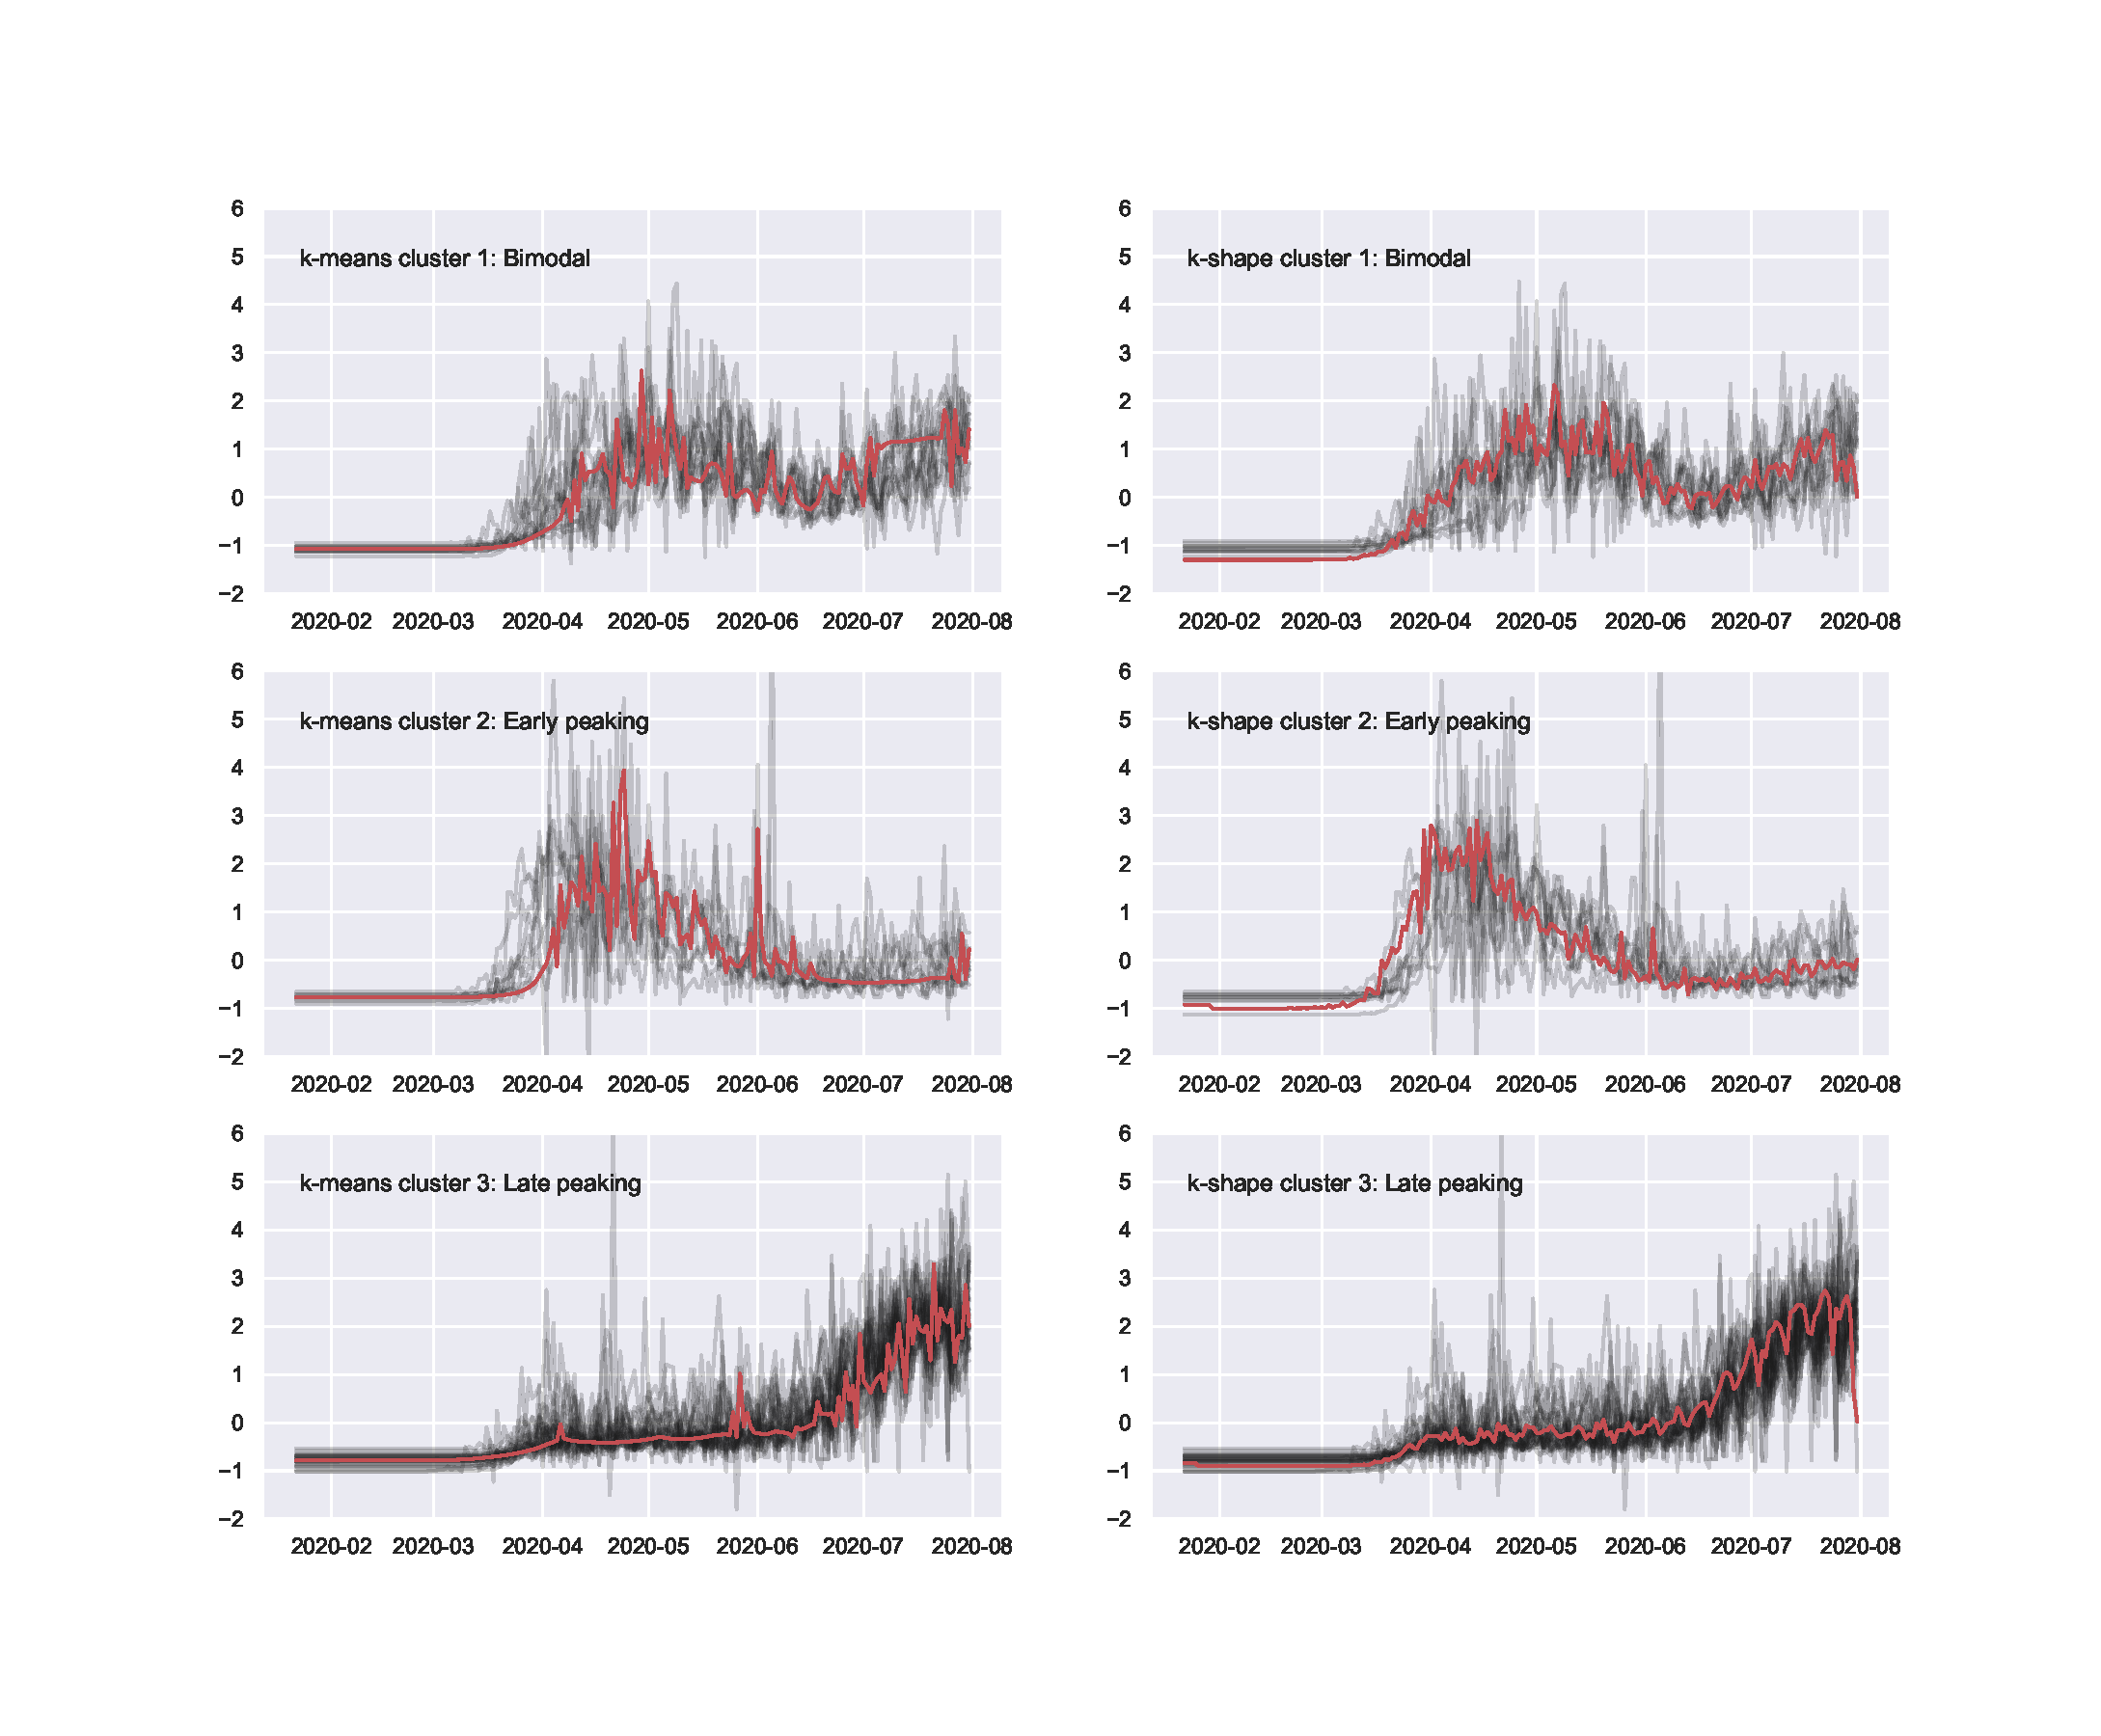
\includegraphics[width=\linewidth]{figures/side-by-side}
	\centering
	\caption{Mutually consistent clusters (rows) between the k-means and k-shape cluster algorithms. Data is time adjusted and barycenters are displayed in red.}
	\label{fig:side-by-side}
\end{figure}

The data set described in Section~\ref{sub:source_data} has been separated into three clusters. As Figure~\ref{fig:side-by-side} shows, there are three distinctly characterisable patterns based on the barycenters:

\begin{enumerate}
	\item Late peaking (k-means cluster 1, k-shape cluster 1): states in this cluster typically have a steady, consistent pattern affected only by weekly periodicities, and begin to surge around mid-June 2020.
	\item Early peaking (k-means cluster 2, k-shape cluster 2): states in this cluster display a rapid-onset initial peak in April to May 2020, thereafter tapering off. 
	\item Bimodal (k-means cluster 3, k-shape cluster 3): within this cluster, states appear to exhibit a steady number of cases and the beginnings of a bimodal distribution over time, with a peak in April-May 2020 that subsides in June, then follows on to another rise in July and August.
\end{enumerate}

\begin{figure}
	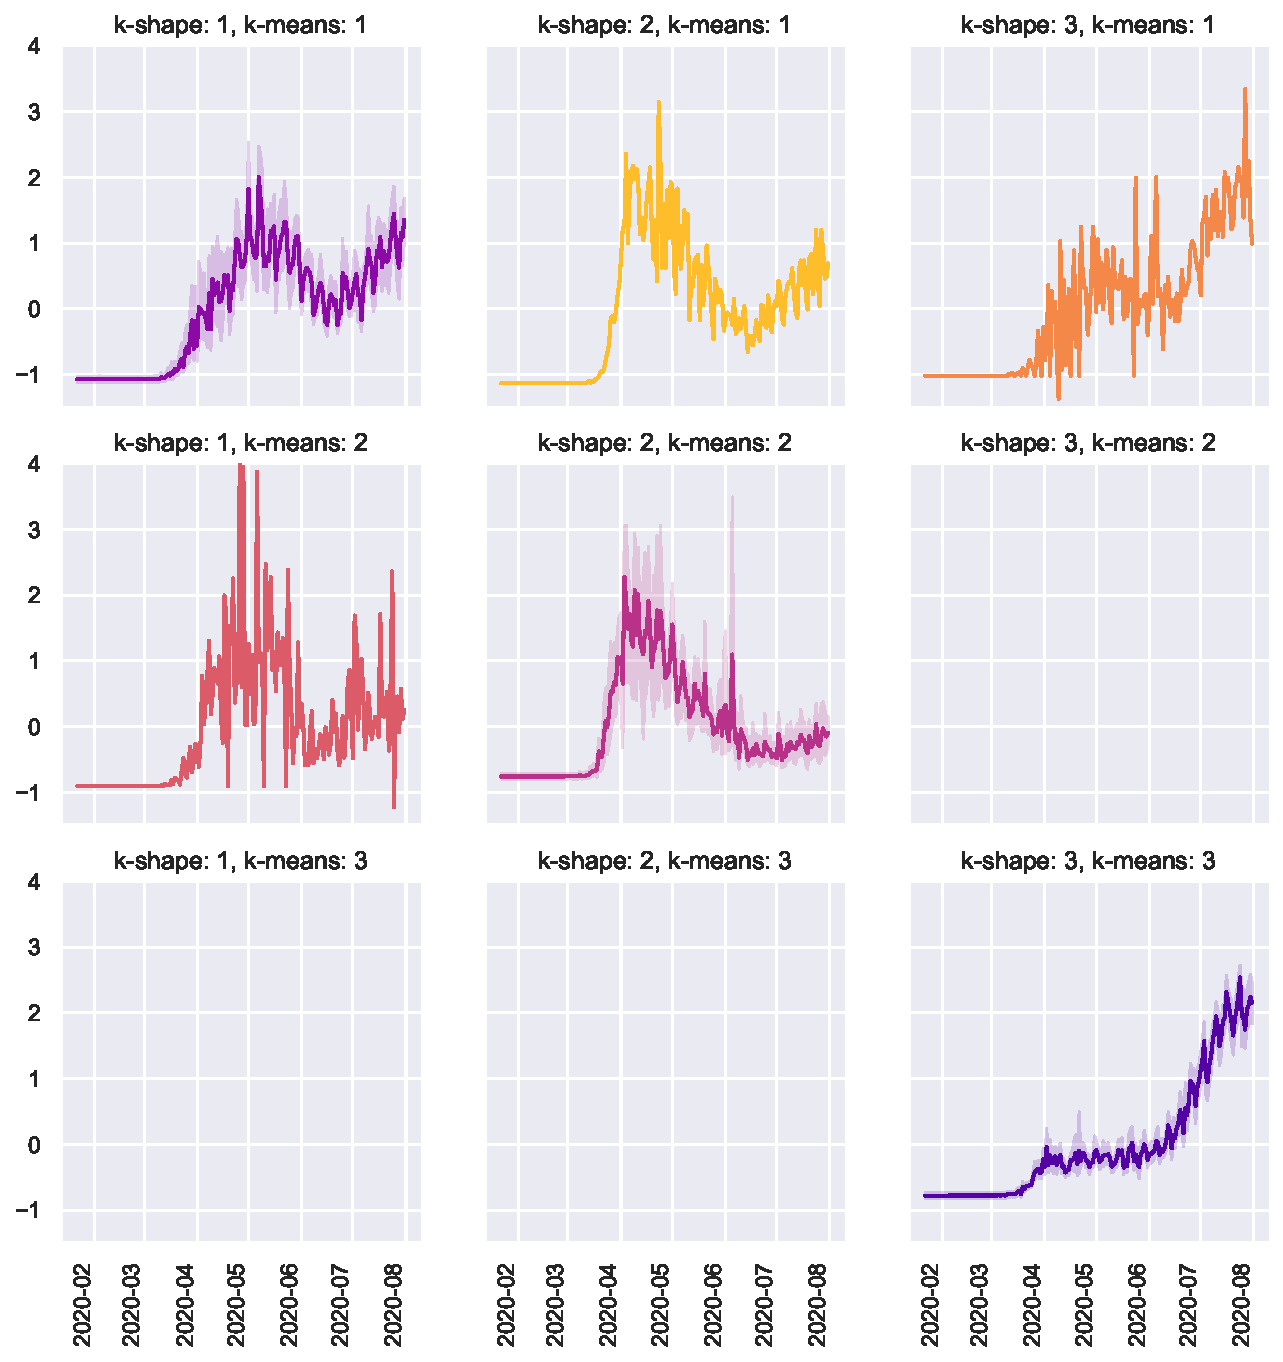
\includegraphics[width=0.8\linewidth]{figures/k-combinations}
	\centering
	\caption{Combined time traces of k-means and k-shape classifications for the major consensus groups. Bimodal behaviour accounts for 21\% of states, early-peaking behaviour covers 17\% and late-peaking, ascending behaviour accounts for over half (56\%) of states. Three states do not fall within the major consensus groups.}
	\label{fig:k_combinations}
\end{figure}

The geographical distribution of the permutation of k-means and k-shape classifications merits mention. As Figure 

% subsection clustering_time_dynamics_of_disease_prevalence (end)

\subsection{Cross-cluster agreement} % (fold)
\label{sub:cross_cluster_agreement}

\begin{figure}
	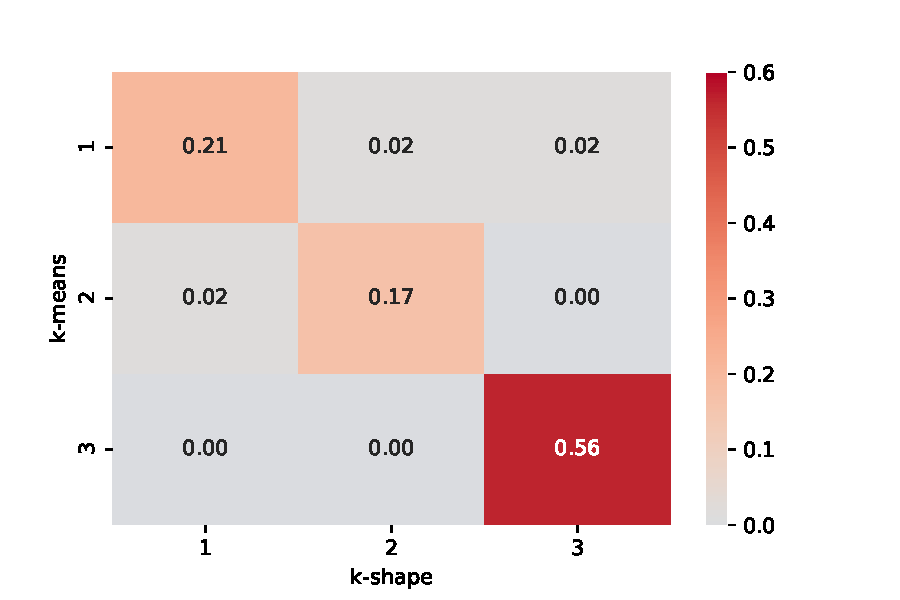
\includegraphics[width=0.5\linewidth]{figures/inter-classifier}
	\centering
	\caption{Inter-classifier agreement between k-shape (\texttt{k-shape}) and soft-DTW k-means (\texttt{kmeans}) classification.}
	\label{fig:inter_classifier}
\end{figure}

In order to ascertain cross-cluster agreement, the Adjusted Rand Index (ARI) was used to quantify consensus between the k-shape and soft-DTW k-means classifiers.\cite{hubert1985comparing} This index, first proposed by Hubert and Arabie in 1985, is symmetric, thus it can be used to identify consensus between clusters with different metrics. At 0.864, the ARI indicates strong concurrence between the soft-DTW k-means and the k-shape classifiers.

Cross-cluster agreement is illustrated in Figure~\ref{fig:inter_classifier}. As it is evident therefrom, over half of the states fall into the late-peaking (k-means cluster 3, k-shape cluster 3) category, with relatively few cases and no pronounced peaks until June 2020, after which the data evidences an oscillating but gradually increasing case count. 

% subsection cross_cluster_agreement (end)

% section results (end)

\section{Discussion} % (fold)
\label{sec:discussion}

k-shape and soft-DTW k-means classification strongly concur in identifying the three fundamental behavioural clusters of confirmed COVID-19 case count in the 48 states of the continental United States: a bimodal pattern, an early peaking pattern and a late, slower pattern that is largely stationary until approx. June 2020, then displays a rapid rise of cases.

\begin{figure}
	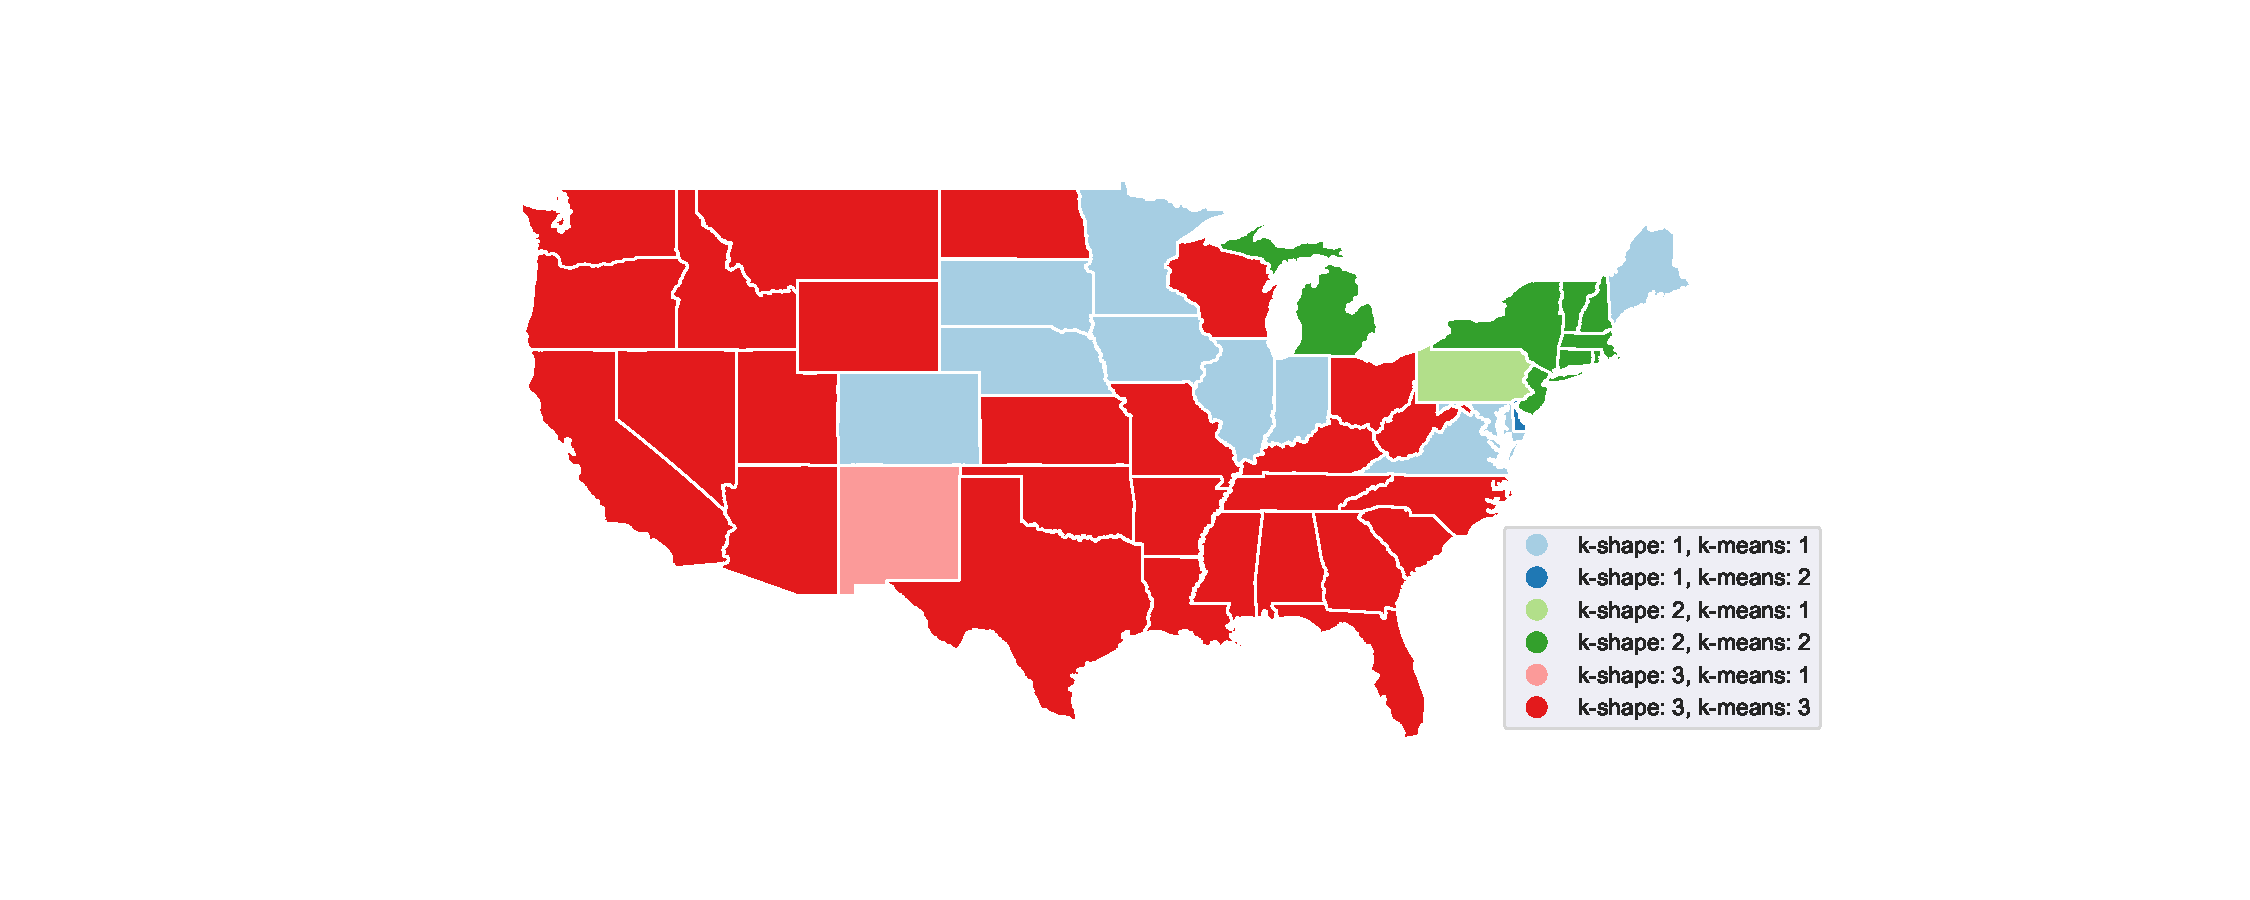
\includegraphics[width=\linewidth]{figures/branch_choropleth}
	\centering
	\caption{Choropleth map of the United States displaying the permutations of k-shape and soft-DTW k-means clustering results by state.}
	\label{fig:choropleth}
\end{figure}

The geographical distribution of these is worth noting. As Figure~\ref{fig:choropleth} shows, most of the area of the continental United States currently follows the late peaking regime, and these states are currently poised to experience further growth in case counts. Only a few states (green shades) have followed an early outbreak by a significant reduction in cases and no further resurgence, which may be considered evidence of successful mitigation/suppression efforts on their part. Finally, a number of states (blue shades) have experienced early outbreaks and are exhibiting a bimodal pattern, whereby an initial surge in April to late May 2020 has been followed not by successful suppression but a reduction followed by yet another uptick in the number of reported cases of COVID-19.

As this paper has shown, time series clustering that allows for finding commonalities between time series that are by necessity out of synchrony can be helpful in illuminating geographical and regional patterns of disease dynamics. In particular, by using two different methods -- a soft-DTW based, time-shifted k-means classifier and the correlation-based k-shape classifier --, the significant consensus between such classifications has been demonstrated where the number of confirmed COVID-19 cases in the continental United States is concerned. 

Thus, by identifying the case count response, we can recognise different internally consistent clusters of case count progression over time. This may assist in understanding the governing patterns and dynamics of the SARS-CoV-2 pandemic, and assist in tailoring responses to the needs of individual areas and communities based on the temporal patterns of epidemic dynamics they exhibit.

% section discussion (end)

\section*{Competing interests} % (fold)
\label{sec:competing_interests}

The author declares no competing interests.

% section competing_interests (end)

\section*{Supplementary data} % (fold)
\label{sec:supplementary_data}

All simulations, code and data are available on Github and under the DOI \texttt{tbc}. Shape files for the choropleth diagram in Figure~\ref{fig:choropleth} have been obtained from the United States Census Bureau, and are included in the data set noted above.

% section supplementary_data (end)

\bibliography{bibliography}

\end{document}
